\documentclass[12pt]{article}
\usepackage[spanish]{babel}
\usepackage[utf8]{inputenc}
\usepackage{amsmath}
\usepackage{listings}
\usepackage[usenames]{color}
\definecolor{gray97}{gray}{.97}
\definecolor{gray75}{gray}{.75}
\definecolor{gray45}{gray}{.45}
\definecolor{azul1}{RGB}{141,198,163}
\definecolor{azul2}{RGB}{24,107,122}
\definecolor{verde1}{RGB}{44,186,34}
\usepackage{graphicx}
\usepackage{caption}
\usepackage{subcaption}
\usepackage{textcomp}
\lstset{
		frame=Ltb,
		framerule=1pt,
		framextopmargin=5pt, %margen de arriba
		framexbottommargin=5pt, %margen de abajo
		framexleftmargin= -2pt, %separacion del margen izquierdo
		framesep=2pt,
		rulesep=0.2pt,
		backgroundcolor=\color{gray97},
		rulesepcolor=,
        tabsize=4,
        rulecolor=\color[RGB]{106, 182, 217}, %AZUL
        upquote=true,
        aboveskip={1.5\baselineskip}, %despues de la linea de texto
        columns=fixed,
        showstringspaces=false,
        extendedchars=true,
        breaklines=true,
        prebreak = \raisebox{0ex}[0ex][0ex]{\ensuremath{\hookleftarrow}},
        showtabs=false,
        showspaces=false,
        showstringspaces=false,
        basicstyle=\scriptsize\ttfamily\color[RGB]{39, 100, 46}, %Numeros de lineas, simbolos, puntos y coma y demas
        identifierstyle=\ttfamily\color[RGB]{56, 140, 189}, %variables
        commentstyle=\color[RGB]{62, 179, 101}, %comentarios
        stringstyle=\color[RGB]{247, 165, 42}, %impresiones
        keywordstyle=\bfseries\color[RGB]{237, 118, 150}, %funciones
        %
		numbers=left,
		numbersep=-7pt, %separacion del numero
		numberstyle=\tiny,
		numberfirstline = false,
		breaklines=true,
		}
\usepackage{graphicx}
\usepackage[colorinlistoftodos]{todonotes}
\usepackage{natbib} %citas bibliograficas estilo APA :p
\usepackage{eso-pic}
\usepackage{avant}
\usepackage[top=2cm,bottom=2cm,left=2.5cm,right=3cm,headsep=8pt,a4paper]{geometry}
\usepackage{fancyhdr}
\pagestyle{fancy}
\fancyhf{}
%\fancyhead[LE,RO]{}
\fancyhead[RE,LO]{Procesamiento de Señales II}
\fancyfoot[CE,CO]{\leftmark}
\fancyfoot[LE,RO]{\thepage}
\renewcommand{\headrulewidth}{2pt}
\renewcommand{\footrulewidth}{1pt}
\usepackage{tabu}
\usepackage{array}
\usepackage{multirow}
\usepackage{amssymb}
\usepackage{makeidx}
\graphicspath{ {images/} }
\usepackage{wrapfig}
\usepackage{enumerate}
\usepackage{amsmath,tikz}
\usetikzlibrary{matrix}
\usepackage{steinmetz}
\newcommand*{\horzbar}{\rule[0.05ex]{2.5ex}{0.5pt}}
\usepackage{calc}
\date{\today}


\begin{document}

\begin{titlepage}
\newcommand{\HRule}{\rule{\linewidth}{0.5mm}} 
\center
\textsc{\LARGE  Benemérita Universidad \\[0.2cm] Autónoma de Puebla}\\[1.5cm] 

\includegraphics[width=4cm]{escudo.jpg}\\[1cm]
\textsc{\Large Facultad de Ciencias de la Electrónica}\\[0.5cm] 
\textsc{\large Licenciatura en Electrónica}\\[0.5cm]
\HRule \\[0.4cm]
{ \huge \bfseries Práctica 4}\\[0.4cm] 
\HRule \\[1.5cm]
\begin{minipage}{\textwidth}
\center 

\emph{Profesor:} \\
Fernando López Marcos \\[1cm]

\begin{tabular}{ll}
\emph{Alumnos:} & \emph{Número de Matrícula:}\\
Hanan Ronaldo Quispe Condori  & 555010653 \\
Erick Sandro Niño García & 201631150\\
Carlos Alfredo Vega Aguilar & 201632131 \\
\end{tabular}
\end{minipage}\\[2cm]
\today
\end{titlepage}

%\newpage
%~\vfill
%\thispagestyle{empty}
%\begin{figure}[hbtp]


%\includegraphics[width=4cm]{IMAGENES/motordc}
%\end{figure}
%\noindent \textsc{Trabajo Encargado: Problemas en MatLab \\ Máquinas Eléctricas \\ Universidad Nacional de San Antonio abad del Cusco}\\
%noindent \textsc{Ingeniería Electrónica }\\
%\noindent \textit{Tercera revisión, \today}

%\tableofcontents indice bloqueado xD

\newpage

\section{Introducción}
Los filtros son una herramienta muy útil en el procesamiento de señales y sirven, entre otras cosas, para 2 actividades principales: Separar señales y restaurar (corregir, limpiar, arreglar) señales.
\\
Existen dos grandes tipos: digitales y analógicos. Los filtros analógicos son baratos y rápidos, pero los filtros digitales tienen mucho mejor desempeño que los analógicos. De los filtros digitales implementados en el dominio del tiempo, se encuentran dos tipos: FIR e IIR.
\\
Los filtros IIR presentan una respuesta al impulso que decae en amplitud infinitamente (Infinite Impulse Response). Se caracteriza por ser expresado por ecuaciones recursivas del tipo:
$$b_1y[n] = a_1 x[n] +a_2 x[n-1]  + ... + a_N x[n-N+1]-(b_2y[n-1]+b_3y[n-2]+...+b_My[n-M+1])$$
Existen distintos tipos de metodologías para el diseño de filtros IIR, uno de ellos es la implementación de la transformación Bilineal o de Tustin a partir de la función de transferencia de un filtro analógico.

\section{Objetivos}
Que el alumno utilice la transformación bilineal para el diseño de un filtro IIR a través de la función de transferencia de un filtro analógico.

\section{Desarrollo}
\textbf{Paso 1.} Se obtiene la función de trasnferencia del filtro analógico de la práctica 3.\\\\ Para esto se usa LCK. El diagrama esquemático del circuito se muestra en la figura 1.

\begin{figure}[h]
        \centering
        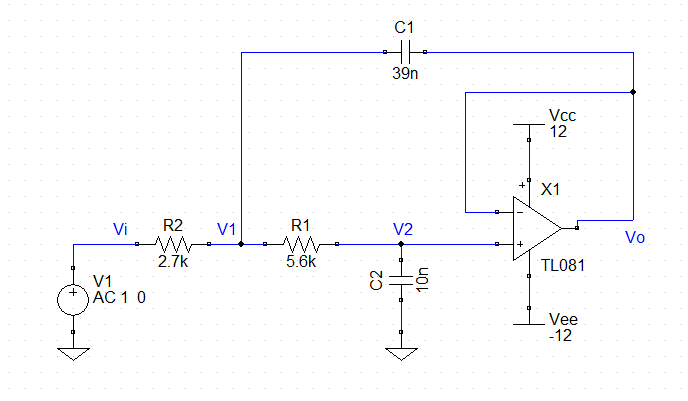
\includegraphics[width=14cm, height=6cm]{im4.PNG}
        \caption{Diagrama esquemático del filtro analógico}
\end{figure}

El sistema de ecuaciones a resolver, obtenido de la figura 1, es el siguiente
$${\frac {{\it V1}-{\it Vi}}{{\it R2}}}+ \left( {\it V1}-{\it Vo}
 \right) s{\it C1}+{\frac {{\it V1}-{\it V2}}{{\it R1}}}=0
$$
$${\frac {{\it V2}-{\it V1}}{{\it R1}}}+{\it V2}\,s{\it C2}=0$$
Donde $Vo$ es el voltaje de salida y $Vi$ es el voltaje de entrada en el filtro. Resolviendo el sistema de ecuaciones nos queda (1)
\begin{equation}
  G=  \left( {\it C1}\,{\it C2}\,{\it R1}\,{\it R2}\,{s}^{2}+{\it C2}\,{
\it R1}\,s+{\it C2}\,{\it R2}\,s+1 \right) ^{-1}
\end{equation}
Donde $G$ esta definido como $\frac{Vo}{Vi}$. Por lo tanto $G$ es la función de transferencia del filtro analógico. Los valores propuesto son 
$${\it C1}={\frac {39}{1000000000}}\text{F}\quad {\it C2}={\frac {1}{100000000}}\text{F}\quad {\it R1}=5600\Omega\quad {\it R2}=2700\Omega $$
Entonces sustituyendo los valores propuestos en la función de transferencia $G$ nos queda (2)
\begin{equation}
    G=\left(  0.000000005896800000\,{s}^{2}+ 0.00008300000000\,s+ 1.0
 \right) ^{-1}
\end{equation}
La respuesta en frecuencia de $G$ se muestra en la figura 2.
\begin{figure}[h]
        \centering
        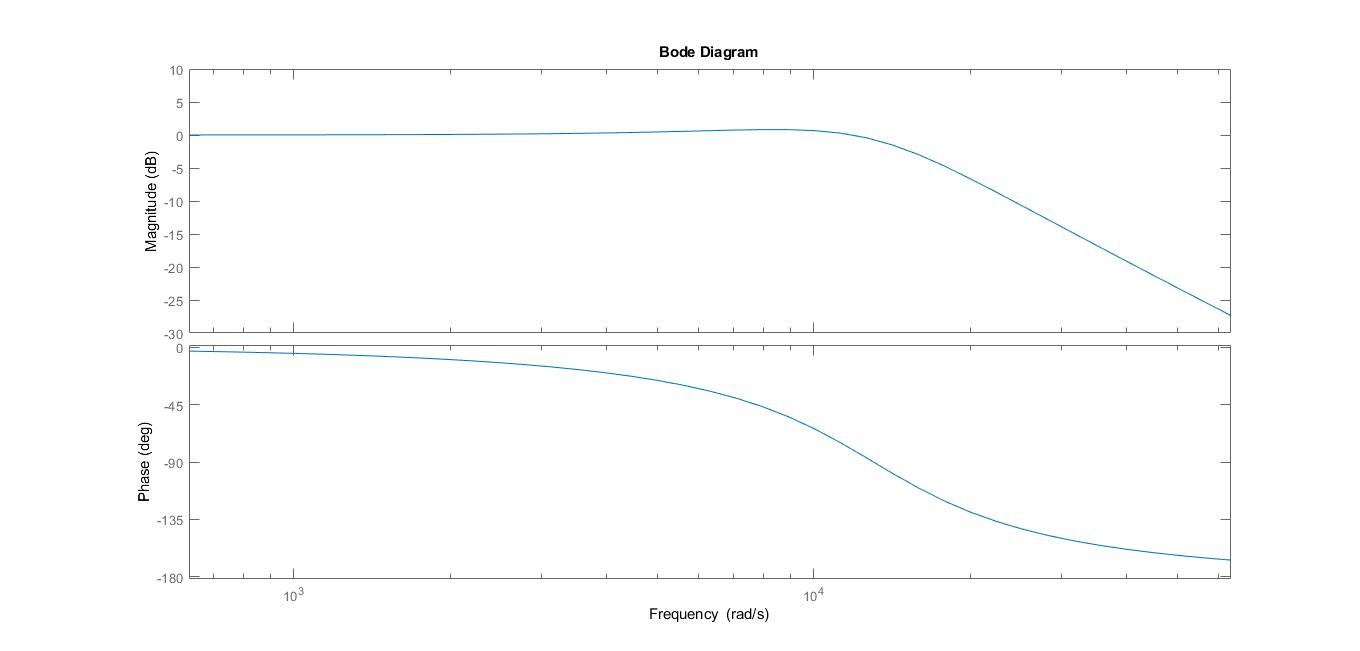
\includegraphics[width=14cm, height=6cm]{im1.jpg}
        \caption{Respuesta en frecuencia de $G$}
\end{figure}

\textbf{Paso 2.}Se obtiene la función de transferencia en tiempo discreto de $G$\\\\
Sustituyendo (3) en (1) nos queda (4) la función de trasnferencia $Gd$ en tiempo discreto.
\begin{equation}
    s=2\,{\frac {z-1}{T \left( z+1 \right) }}
\end{equation}
'\begin{equation}
    Gd={\frac {{T}^{2} \left( 1+z \right) ^{2}}{ B {z}^{2}+ \left( -8\,{\it C1}\,{\it C2}\,{\it R1}\,{
\it R2}+2\,{T}^{2} \right) z+4\,{\it C1}\,{\it C2}\,{\it R1}\,{\it R2}
+2\,{\it C2}\,{\it R1}\,T+2\,{\it C2}\,{\it R2}\,T+{T}^{2}}}
\end{equation}

Donde $B$ es
$$B=\left( 4\,{\it C1}\,{\it C2}
\,{\it R1}\,{\it R2}-2\,{\it C2}\,{\it R1}\,T-2\,{\it C2}\,{\it R2}\,T
+{T}^{2} \right)$$
La función de transferencia en tiempo discreto $Gd$ con un tiempo de muestreo de $T=\frac{1}{44100}$ segundos y con los valores propuestos en el paso 2 es (5)

\begin{equation}
Gd=\frac{0.01845+0.0369z^{-1}+0.01845z^{-2}}{1-1.656z^{-1}+.7298z^{-2}}
\end{equation}

\textbf{Paso 3.} Se compara la respuesta en frecuencia de $G$ y $Gd$\\\\
La respuesta en frecuencia de $G$y $Gd$ se muestra en la figura 3

\begin{figure}[h]
        \centering
        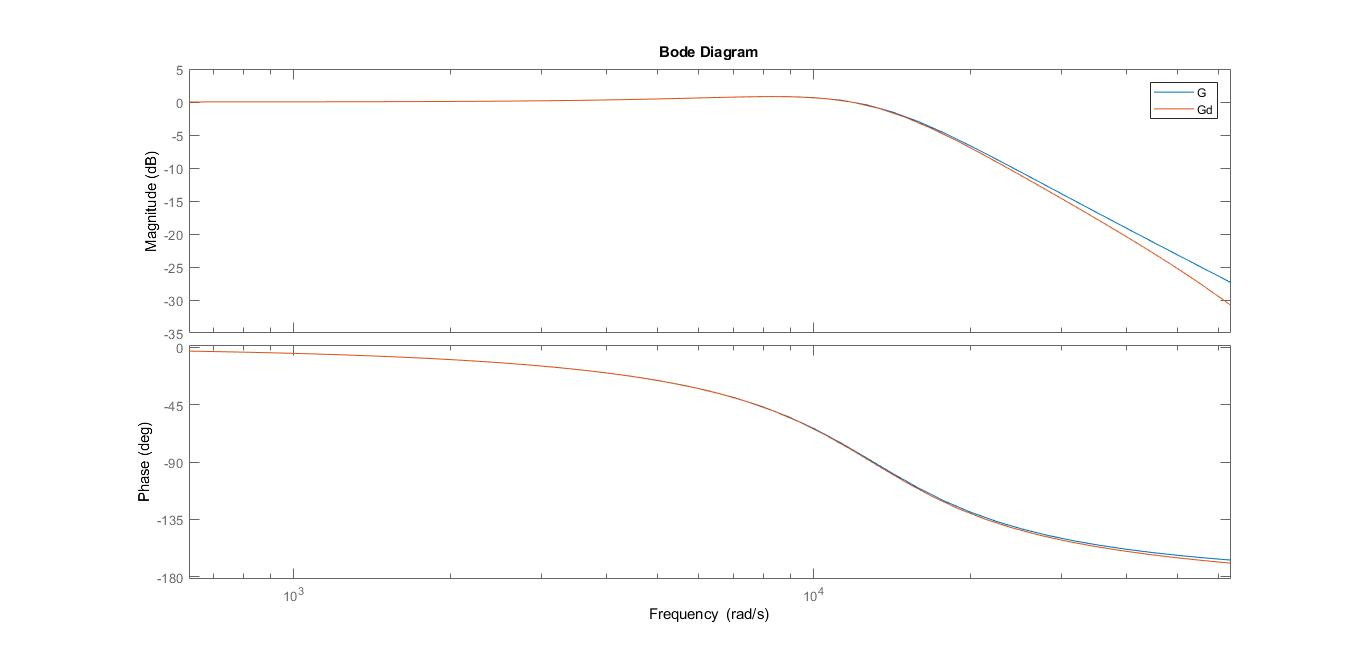
\includegraphics[width=14cm, height=6cm]{im2.jpg}
        \caption{Respuesta en frecuencia de $Gd$}
\end{figure}

\textbf{Paso 4.} Se determina la ecuación en diferencias para implementar el filtro y se analiza su respuesta en frecuencia.\\\\

Para obtener la ecuación en diferencias de la función de trasnferencia $Gd$ se desarrollan los siguientes pasos
$$\frac{Y(z)}{X(z)}=\frac{0.01845+0.0369z^{-1}+0.01845z^{-2}}{1-1.656z^{-1}+.7298z^{-2}}$$\\
$$Y(z)(1-1.656z^{-1}+.7298z^{-2})=X(z)(0.01845+0.0369z^{-1}+0.01845z^{-2})$$\\
$$Y(z)-1.656z^{-1}Y(z)+.7298z^{-2}Y(z)=0.01845X(z)+0.0369z^{-1}X(z)+0.01845z^{-2}X(z)$$\\
Aplicando la transformada $Z$ inversa obtenemos la ecuación de diferencias (6)
\begin{equation}
    y(n)-1.656y(n-1)+.7298y(n-2)=.01845x(n)+.0369x(n-1)+.01845x(n-2)
\end{equation}

Con los coeficientes de la ecuación de diferencias se implementa el filtro en matlab (ver apéndices) y se obtiene la respuesta en frecuencia. La respuesta en frecuencia se muestra en la figura 4.

\begin{figure}[h]
        \centering
        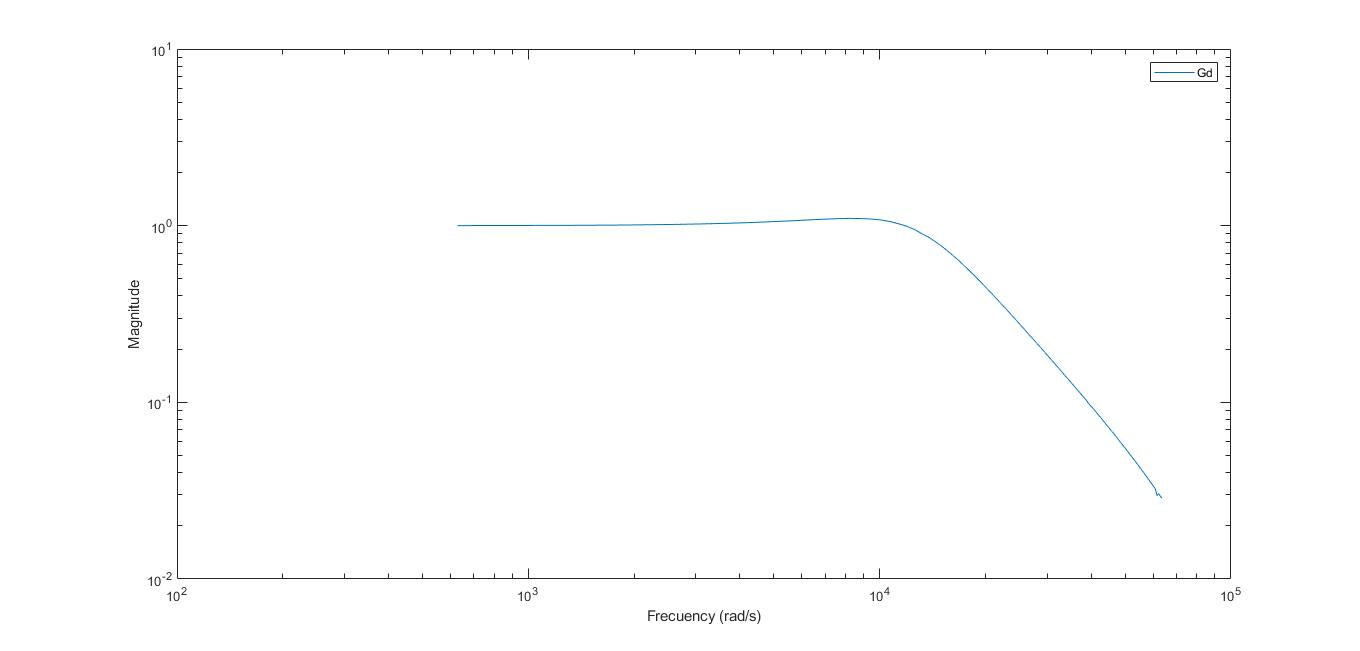
\includegraphics[width=14cm, height=6cm]{im3.jpg}
        \caption{Respuesta en frecuencia del filtro $Gd$ implementado en un rango de $100(2\pi)$ a $10000(2\pi)$ rad/s}
\end{figure}
\newpage
\section{Cuestionario}
\textbf{Describa las diferencias entre las gráficas de las respuestas en frecuencia obtenidas en los pasos 2 y 4.}
\\
\\
En la figura 3, se muestra esta comparativa de manera muy clara. Donde la línea de color azul corresponde al comportamiento del filtro analógico y la línea de color naranja pertenece al filtro digital. Nótese que en la banda de paso, las líneas están practicamente sobrepuestas mostrando un comportamiento congruente, incluso en la banda de transición las líneas siguen sobrepuestas. Comienzan a separarse aproximadamente a los -8dB y conforme la frecuencia sigue aumentando, las gráficas difieren cada vez más. Es hasta después de los 14kHz que la diferencia se hace significante con una separación de 10dB mostrando mejor atenuación el filtro digital. Tomando en cuenta que la frecuencia de corte de los filtros es de 2kHz y la diferencia entre las atenuaciones se ve reflejada hasta los 14kHz, puede pensarse que tener diferencias 12kHz después de la de corte es un mal resultado. Pero lo que decidirá si el filtro es bueno o malo, son de las aplicaciones a las que será sometida.
\\
En la fase se tienen diferencias mínimas. 
\\
\\
\textbf{Verifique el rizado en las bandas de paso y rechazo de su filtro y compara con las características planteadas inicialmente.}
\\
\\
En la banda de paso se tiene un pico máximo de 0.825dB para ambos filtros, ya que como se mencionó, en este punto ambas gráficas están sobrepuestas. Este valor de dB es el mismo que se obtuvo en la simulación en SPICE del filtro analógico y tener esta congruencia es un resultado favorable. Para la banda de rechazo, de manera semejante a la de paso, los comportamientos de las simulaciones de SPICE y el obtenido para el filtro digital son bastante semejantes teniendo incluso una mejoría para el digital a frecuencias superiores a 10kHz.
\\
\\
\section{Conclusiones}
Los filtros digitales suelen ser más utilizados cuando se requieren trabajos más pesados como en un estudio de grabación ya que se requieren filtrados más estrictos para obtener sonidos limpios y sin ningún tipo de ruido. Para obtener filtros más eficientes, se requiere incrementar el orden de dicho filtro, y en filtros analógicos, un orden mayor requiere más componentes pasivos y a menos que tengan un comportamiento casi ideal, se tendrán pérdidas que a la larga serán significantes, además que se requiere darle mantenimiento, suministrar energía, la velocidad de trabajo dependerá de la calidad de los componentes, etc. En cambio, se requieren menos recursos para obtener filtros digitales eficientes y son más rápidos. Por lo anterior, se hace funcional conocer la metodología para diseñar filtros digitales a partir de fitros analógicos entendiendo que si este proceso se hace correctamente, no habrán diferencias significativas en su comportamiento.
\section{Apéndice}
\textbf{Código implementado para la comparación del filtro Analógico con el filtro Digital}
\lstinputlisting[language=Matlab]{LPF_Test_Equipo2.m}
\end{document}
